\documentclass{standalone}
\usepackage{tikz}
\usepackage{tkz-euclide}
\usepackage{ctex}
\pagestyle{empty}
\setCJKmainfont{Noto Serif CJK SC}
\usepackage{siunitx,chemmacros,chemfig}
\setchemfig{bond offset = 0pt}
\chemsetup[orbital]{
  overlay,
  opacity=0.5,
  sp/scale=1.2,
  s/color=blue!50,
  s/scale=1.0
}
\begin{document}
\small
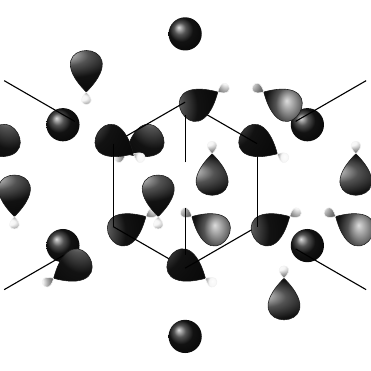
\begin{tikzpicture}
  \useasboundingbox(-2.0,-2)rectangle(2.0,2);
  \node {
  \chemfig{*6(
    ({\orbital[angle=90]{sp}}{\orbital[angle=210]{sp}}{\orbital[angle=330]{sp}}-[,0.7]\orbital{s})
    -({\orbital[angle=30]{sp}}{\orbital[angle=150]{sp}}{\orbital[angle=270]{sp}}-[,0.7]\orbital{s})
    -({\orbital[angle=90]{sp}}{\orbital[angle=210]{sp}}{\orbital[angle=330]{sp}}-[,0.7]\orbital{s})
    -({\orbital[angle=30]{sp}}{\orbital[angle=150]{sp}}{\orbital[angle=270]{sp}}-[,0.7]\orbital{s})
    -({\orbital[angle=90]{sp}}{\orbital[angle=210]{sp}}{\orbital[angle=330]{sp}}-[,0.7]\orbital{s})
    -({\orbital[angle=30]{sp}}{\orbital[angle=150]{sp}}{\orbital[angle=270]{sp}}-[,0.7]\orbital{s})-)
  }
  };
\end{tikzpicture}
\end{document}